\section{Introduction}
In Chapter \ref{ch:OverView}, we saw various elements of VHDL language. In this chapter, we will discuss the `Dataflow' modeling style in detail; in which functionality of the entity is described using `concurrent statements' (without defining the structure of the design). 


\section{Delay in signal assignments}
In Chapter \ref{ch:OverView}, we saw that concurrent statements do not execute sequentially i.e. order of statements do not matter in concurrent statements. More precisely, these statements are `event triggered' statements i.e. these statements execute whenever there is any event on the signal, as discussed in Listing \ref{vhdl:deltaDelayEx} and \ref{vhdl:afterDelay}.

Remember that, lines 15 and 16 in Listing \ref{vhdl:deltaDelayEx} and \ref{vhdl:afterDelay} are the example of signal assignments. In this section, two types of delays in signal assignments, i.e. `delta delay ($\Delta t$)' and `delay using `after' statement', are discussed. 

\subsection{Delta delay}
If `no delay' or delay of `0 ns' is specified in the statement, then delta delay is assumed in the design. These two delays are shown in Listing \ref{vhdl:deltaDelayEx} which is explain below. 
\begin{explanation}[Listing \ref{vhdl:deltaDelayEx}]
	In this listing, `x' and `z' are the input and output ports respectively, whereas `s' is the signal. In line 15, delay is not defined explicitly; whereas in Line 16, 0 ns delay is defined. Hence, in both the cases `delta delay ($\Delta t$)' is assumed which is explained in next paragraph. 
	
	As explained before, concurrent statements execute whenever there is any change in the signals; therefore line 16 will be executed, when there is any change in the input `x'. This statement will execute in $\Delta t$ time. Hence, the value of signals `s' will be changed after $\Delta t$ time. Since the value of `s' is changed, therefore in next $\Delta t$ time, line 15 will execute and the value of `z' will be changed. 
	
	In the other words, the code will execute `two times' in $2\Delta t$ time to complete the signal assignments; in first $\Delta t$ time, value of `s' will change and in next $\Delta t$ time, the value of `s' will be assigned to `z'. In general, code will execute until there is no further change in the signals. Also, delta delay is very small and can not be seen in simulation results as illustrated in Fig. \ref  {fig:deltaDelayEx}.	Further, in the figure, all the values i.e. `x', `s' and `z' are changed at the same time, which indicates that delta delay is very small and can not be observed. 
	
	\begin{noNumBox}
	 Note that	multiple signal assignments are not allowed in VHDL, as shown in line 17 of Listing \ref{vhdl:deltaDelayEx}. Here, signal assignment for `z' is done twice i.e. line 15 and 17. If we uncomment the line 17, then model will be invalid and error will be generated. 
	\end{noNumBox}
\end{explanation}

\lstinputlisting[
language = Vhdl,
caption    = {Delta delay},
label      = {vhdl:deltaDelayEx}
]{deltaDelayEx.vhd}

\begin{figure}[!h]
	\centering
	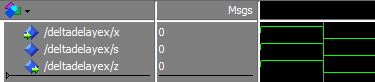
\includegraphics{deltaDelayEx}
	\caption{Delta delay}
	\label{fig:deltaDelayEx}
\end{figure}

\subsection{Delay with `after' statement}
We can assign the desired delay in the signal assignment statement as shown in lines 15 and 16 of Listing \ref{vhdl:afterDelay}. Here signal `s' is assigned after the delayed of 1 ns (line 15), then the value of `s' is assign to `z' after 1 ns (line 16). Hence the output `z' will be delay by 2 ns with respect to `x' as shown in Fig. \ref{fig:afterDelay} using vertical red lines (which show the propagation of value `1'). Also, horizontal red lines for `s' and `z' show that these signals are uninitialized for that time period (because values are assigned after 1 and 2 ns respectively). 


\lstinputlisting[
language = Vhdl,
caption    = {Specify delay using `after'},
label      = {vhdl:afterDelay}
]{afterDelay.vhd}

\begin{figure}[!h]
	\centering
	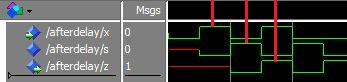
\includegraphics{afterDelay}
	\caption{Delay}
	\label{fig:afterDelay}
\end{figure}

\section{Concurrent signal assignments}
Similar to `if' statement in behavioral modeling, `dataflow' modeling provides two signal assignments i.e. `Conditional signal assignment' and `Selected signal assignment'. Multiplexer is designed using these two assignments. 

Multiplexer is a combinational circuit which selects one of the many inputs with selection-lines and direct it to output. Table \ref{tbl:Multiplexer} illustrates the truth table for $4\times 1$ multiplexer. Here `i0 - i3' the input lines, whereas `s0' and `s1' are the selection line. Base on the values of `s0' and `s1', the input is sent to output line, e.g. if s0 and s1 are 0 then i0 will be sent to the output of the multiplexer.

\begin{table}[!h]
	\centering
	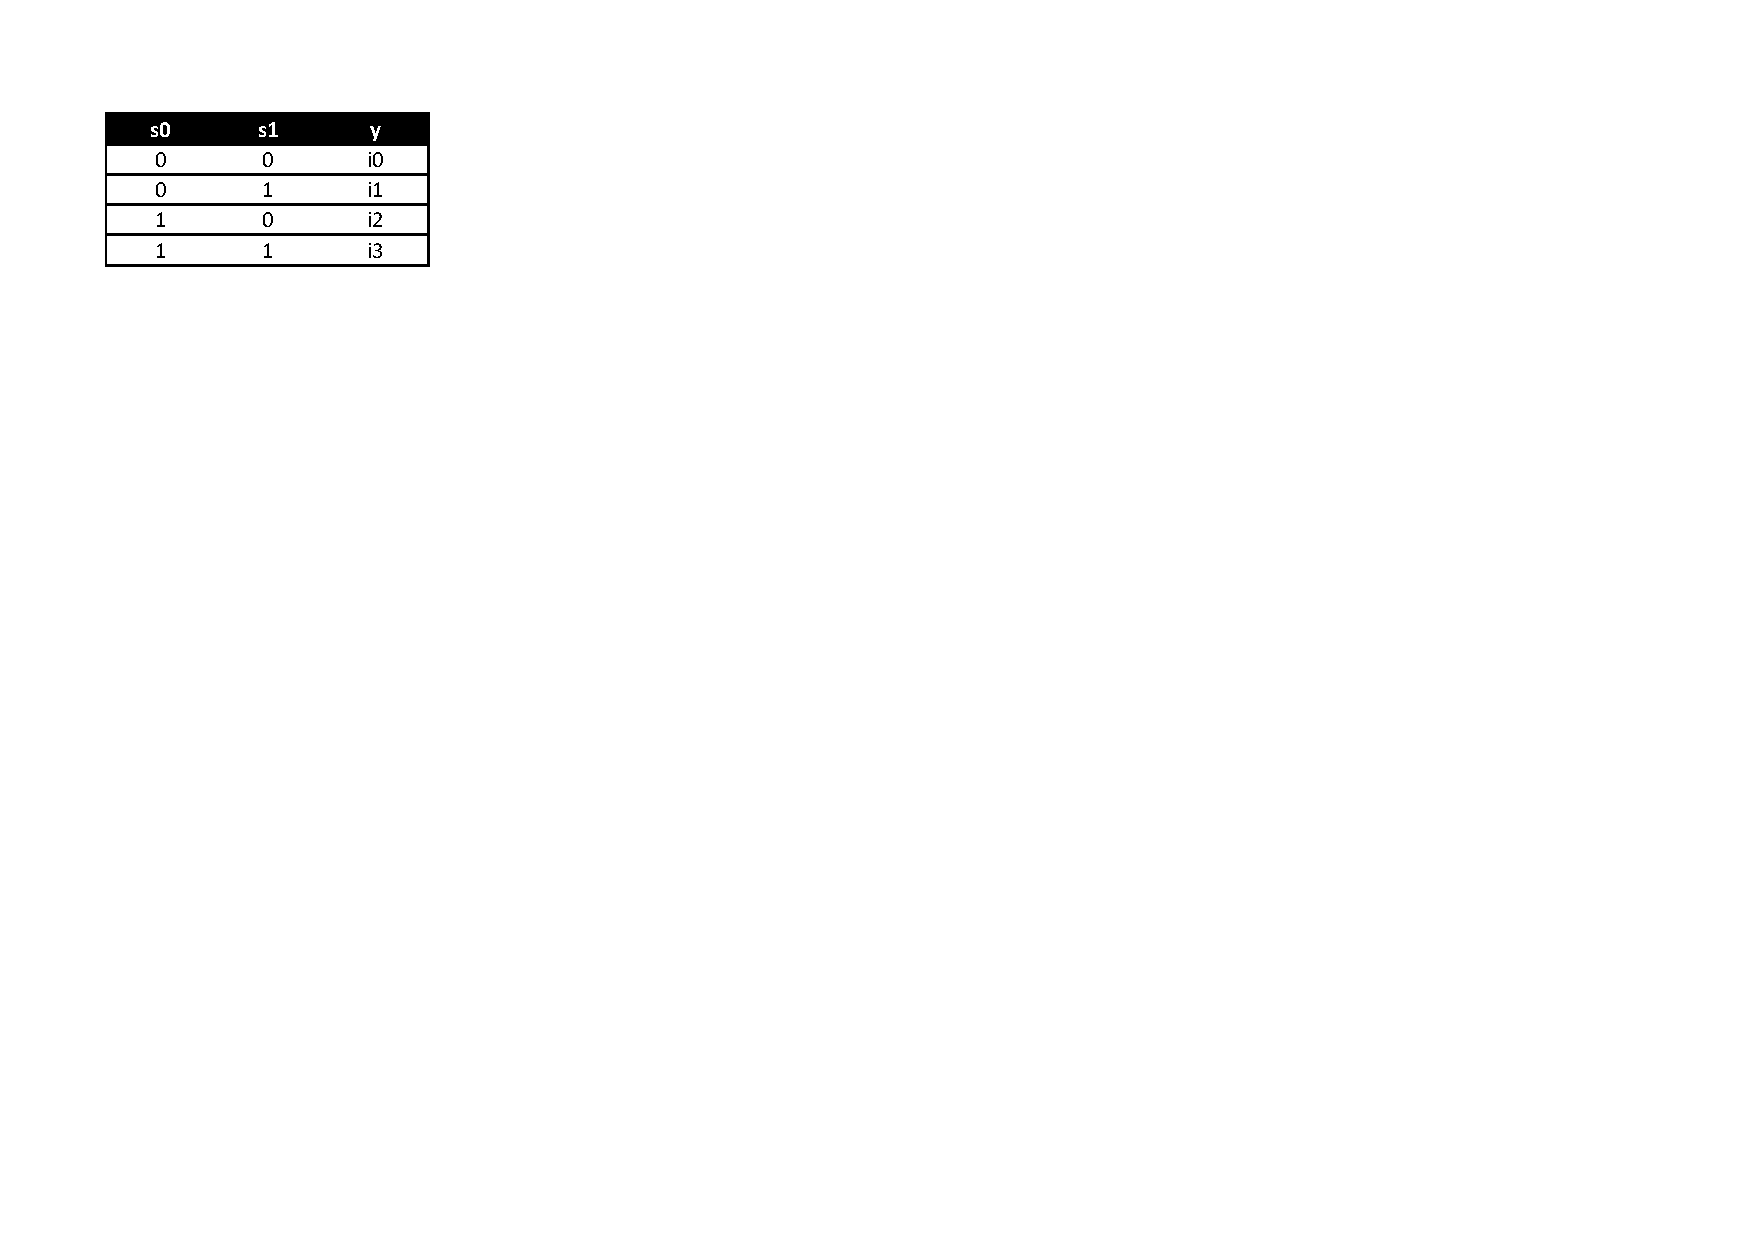
\includegraphics{tableMultiplexer}
	\caption{Truth table of 4$\times$1 multiplexer}
	\label{tbl:Multiplexer}
\end{table}


\subsection{Conditional signal assignment}

Syntax for conditional signal assignment is shown in lines 15-18 of Listing \ref{vhdl:multiplexerEx}, where `when' and `else' keywords are used for assigning the value to output port `y'. Conditional signal assignments are implemented using `2$\times$1' multiplexer as shown in Fig. \ref{fig:multiplexerEx}. Here, three `2$\times$1' multiplexer (i.e. y$\sim$0, y$\sim$2 and y$\sim$4) are used to design the `4$\times$1' multiplexer.

\lstinputlisting[
language = Vhdl,
caption    = {Multiplexer using Conditional signal assignment},
label      = {vhdl:multiplexerEx}
]{multiplexerEx.vhd}


\begin{figure}[!h]
	\centering
	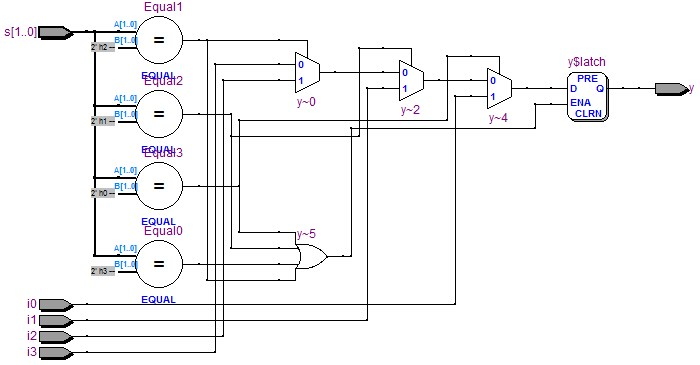
\includegraphics[width=0.8\textwidth]{multiplexerEx}
	\caption{Multiplexer using Conditional signal assignment}
	\label{fig:multiplexerEx}
\end{figure}

Fig. \ref{fig:multiplexerExWave} shows the waveform of Listing \ref{vhdl:multiplexerEx}. Here i0, i1, i2 and i3 are set to 1, 0, 1 and 0 respectively. Then simulator is run 4 times for all the combination of `s' i.e. 00, 01, 10 and 11 respectively; and output `y' is assigned the value based on the `s' value e.g if s is `00' then y is assigned with the value of `i0' i.e. 1 etc.  

\begin{figure}[!h]
	\centering
	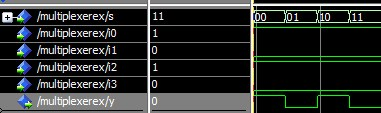
\includegraphics[scale=0.8]{multiplexerExWave}
	\caption{Multiplexer waveform for Listing \ref{vhdl:multiplexerEx} and \ref{vhdl:multiplexerVhdl}}
	\label{fig:multiplexerExWave}
\end{figure}



\subsection{Selected signal assignment}
Syntax for selected signal assignment is shown in lines 15-23 of Listing \ref{vhdl:multiplexerVhdl}, where `with-select' and `when' keywords are used for assigning the value to output port `y'. Unlike conditional signal statement, in selected signal assignment implements the 4$\times$1 multiplexer with 4$\times$1 multiplexer itself as shown in Fig. \ref{fig:multiplexerVhdl}, rather than with multiple 2$\times$1 multiplexer. Further, the waveforms for Listing \ref{vhdl:multiplexerVhdl} is shown in Fig. \ref{fig:multiplexerExWave}.

Note that `unaffected when others' is used in line 23.  `others' is used to avoid the error which is caused by the logics which can not be synthesized,  as mentioned in comments in lines 20-22. Further, `unaffected' is the keyword which does not allow any change in the signal.

\begin{figure}[!h]
	\centering
	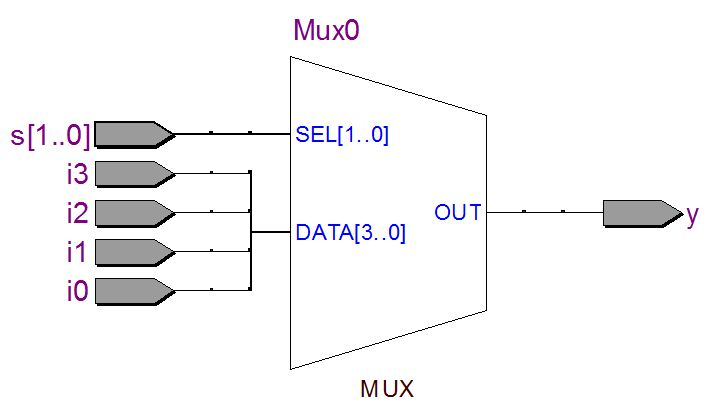
\includegraphics[scale=0.4]{multiplexerVhdl}
	\caption{Multiplexer using Selected signal assignment}
	\label{fig:multiplexerVhdl}
\end{figure}

\lstinputlisting[
language = Vhdl,
caption    = {Multiplexer using Selected signal assignment},
label      = {vhdl:multiplexerVhdl}
]{multiplexerVhdl.vhd}

\section{Conclusion}
In this chapter, we saw various features of Dataflow modeling style. We discussed the delays in VHDL designs. Also, 4$\times$1 multiplexer is implemented using conditional and selected signal assignments. Further, the differences in the designs generated by these two assignments are shown using figures.